\section{Projekt}\label{projekt}

\subsection{\texorpdfstring{Symulacja \autocite{Hartmann:simulation:2005} \autocite{hartmann:2015:bigsim}}{Symulacja  }}\label{symulacja}

Eksperymenty, fizyczne, ekonomiczne lub socjologiczne, w świecie rzeczywistym bywają skomplikowane lub niemożliwe do przeprowadzenia. Symulacja jest procesem umożliwiającym takie eksperymenty poprzez proces reprezentacji świata rzeczywistego jako uproszczonego, abstrakcyjnego modelu. W wielu przypadkach wykorzystywana jest losowość, aby wprowadzić element różnorodności do symulacji. Umożliwia to naukowcom wykorzystanie statystycznych obserwacji do uzupełnienia szczegółów uproszczonego modelu, których nie da się przedstawić w modelu matematycznym lub czynniki ten nie mają bezpośredniego wpływu na badanie. Połączenie losowości z możliwością sterowania warunkami modelu umożliwia generowanie wyników poprzez zapis cyklu uruchomień modelu i statystyczną ich analizę. Obiektem dyskusji w tej pracy są symulacje komputerowe. chociaż historia symulacji sięga daleko przed powstaniem komputerów. Przed komputerami, dużą rolę w symulacjach odgrywało modelowanie matematyczne. W tej dziedzinie cały system jest przedstawiony w postaci zbioru równań, obliczanych dla zadanych parametrów. W kontraście, symulacje opierają się na uruchomieniach modelu, dla których dwa wyniki z tymi samymi warunkami początkowymi mogą być inne. Symulacje komputerowe dzielą się na dwie kategorie. Pierwszą z nich stanowią symulacje modele, w których aktorzy, ludzie lub inne elementy świata rzeczywistego, wchodzą w interakcję z systemem w czasie symulacji. Systemy te są często nazywane systemami ``w pętli'' lub symulacją z ``ludźmi w pętli''. Sztandarowymi przykładem tego typu symulacji są gry komputerowe, interaktywne systemy treningu wojskowego oraz systemy testowania maszyn przemysłowych. Drugą z kategorii są symulacje, w których cały system jest zaprojektowany jako oprogramowanie komputerowe. Wśród nich znajdują się symulacje ze zdarzeniami dyskretnymi, symulacje z czasem dyskretnym oraz symulacje statystyczne/Monte Carlo. Kluczową cechą wyróżniającą metody ``w pętli'' od pozostałych jest wymaganie odpowiedzi w czasie rzeczywistym. Systemy ``w pętli'' muszą odpowiadać w zadanym czasie, aby zewnętrzny obserwator, człowiek lub maszyna, otrzymał odpowiedź na wykonaną akcje. W przeciwieństwie do systemów ``W pętli'', pozostałe systemy generują wyniki symulacji w dowolnych odstępach czasowych.

W symulacjach ze zdarzeniami dyskretnymi, modelowany system jest przedstawiony jako stan i zbiór zdarzeń, które wpływają na niego. Zdarzenia są częściowo uporządkowane wedle czasu, w którym się wydarzyły w modelu. Zdarzenia są przechowywane w uporządkowanej strukturze, jak kolejka, oraz przetwarzane przez algorytm symulacji. Algorytmy oparte o dyskretne zdarzenia implementują pętlę zdarzeń, która przetwarza zdarzenia, dopóki nie zajdzie warunek końcowy. Warunkami stopu może być wyczerpanie kolejki zdarzeń, liczba przetworzonych zdarzeń, upływ czasu w modelu lub warunki opierające się o stan symulacji. Czas jest modelowany jako znacznik czasowy ostatnio przetworzonego zdarzenia. W każdym cyklu iteracji pętli zdarzeń najwcześniejsze zdarzenie jest ściągane z kolejki, aby je przetworzyć. W przypadku gdy jest więcej niż jedno zdarzenie z tym samym znacznikiem czasowym, potrzebne jest atomowe przetwarzanie współbieżnych zdarzeń lub mechanizm decyzyjny, który uporządkuje względem siebie zdarzenia. Aby przetworzyć zdarzenie, stan modelu jest modyfikowany na podstawie zawartości zdarzenia. Taka zmiana może mieć również skutki uboczne, które generują kolejne zdarzenia. W symulacji ze zdarzeniami dyskretnymi przedstawiony jest jedynie czas, w którym zdarzenia są generowane, okres pomiędzy może zostać pominięty, aby zredukować moc obliczeniową potrzebną do pokrycia rzadko wypełnionych przedziałów czasowych.

Symulacja z czasem dyskretnym jest modyfikacją symulacji ze zdarzeniami dyskretnymi. Zamiast skokowego postępu czasu wynikającego z czasu zdarzeń, w tym typie symulacji czas posuwa się o stałą wartość. Wszystkie zdarzenia, które pojawiają się w danym okresie czasu, są traktowane tak jakby wydarzyły się w tym samym momencie. Podejście to ma szereg zalet nad symulacją ze zdarzeniami dyskretnymi. W przypadku dyskretnych zdarzeń, gdy zdarzenia są gęsto rozmieszczone w czasie, symulacja nie może pomijać okresów, co zwiększa zapotrzebowanie na moc obliczeniową. Ten problem nie występuje w symulacji z czasem dyskretnym ze względu na równe odstępy czasu pojawiania się zbioru zdarzeń. Kolejną zaletą wynikającą z tej własności jest brak konieczności utrzymywania globalnej, uporządkowanej struktury danych zdarzeń. Zamiast niej można wykorzystać struktury danych o lepszych właściwościach dostępu do danych, takich jak tablice mieszające. Co więcej, dzięki temu, że w symulacjach z czasem dyskretnym zdarzenia w danym okresie czasu występują jednocześnie, przetwarzanie tego okresu można zrównoleglić. W takim przypadku przetwarzanie można rozdzielić pomiędzy wiele procesów roboczych na zasadzie rozprosz-zbierz (\emph{ang. scatter-gather}).

\subsubsection{\texorpdfstring{Symulacja w grach komputerowych \autocite{vogel:simulation}}{Symulacja w grach komputerowych }}\label{symulacja-w-grach-komputerowych}

\subsubsection{\texorpdfstring{Generatory liczb losowych i pseudolosowych \autocite{Ecuyer:rng} \autocite{Hellekalek:rng} \autocite{Ecuyer:simulation:rng} \autocite{Kneusel2018RandomNA}}{Generatory liczb losowych i pseudolosowych    }}\label{generatory-liczb-losowych-i-pseudolosowych}

Losowość ma wiele zastosowań. Często sprawdzenie wszystkich możliwych przypadków jest niepraktyczne, a losowa próbka pozwoli zbadać typowe zachowanie. Liczby losowe są również wykorzystywane w programach komputerowych, aby sprawdzać efektywność algorytmów. Ponadto, istnieje cała kategoria algorytmów losowych, zwanych też \emph{Monte Carlo}, które opierają swoje działanie na losowości. Szczególnym przypadkiem programów komputerowych, są gry. W nich losowość jest stosowana, aby świat przedstawiony wydawał się bardziej rzeczywisty. Liczby losowe wykorzystuje się do podobnych celów w symulacjach, w których komputer odwzorowuje zjawiska naturalne.
Ciężko określić co jest liczbą losową, bo czy liczba 2 jest losowa? Poprzez losowość rozumiemy \emph{losową sekwencję}.

\begin{quote}
Sekwencją losową \emph{a} \emph{n} liczb nazywamy sekwencję liczb, zawierających się w określonym zbiorze, w której nie da się przewidzieć \(n_{k+1}\) z żadnej kombinacji poprzedzającej \(n_i, i = 0,1,...,k\).
\end{quote}

Można postrzegać losową sekwencję jako generator, który produkuje wartość, kiedy jest o to poproszony, której nie da się przewidzieć na podstawie żadnej z poprzednich wartości.
Procesy losowe są często przedstawiane jako próbkowanie z funkcji rozkładu prawdopodobieństwa. W związku z tym, pomimo faktu, że da się przewidzieć \(n_k\), można stworzyć przybliżenie rozkładu, zbudowanego na podstawie histogramu z wartości próbek pobranych z generatora.

\begin{figure}[htbp]
\centering
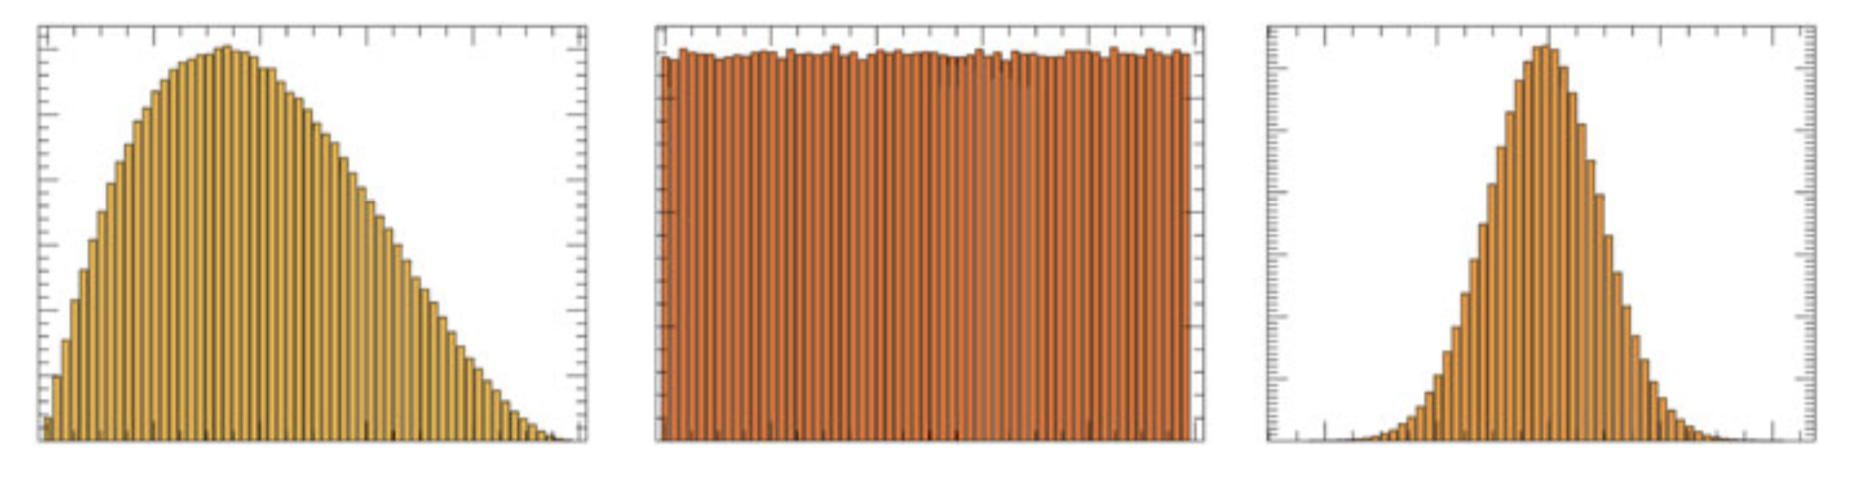
\includegraphics[width=140mm]{graphics/distributions.png}
\caption{Przykładowe rozkłady przedstawiające procesy losowe \autocite{Kneusel2018RandomNA}}
\end{figure}

Zakładamy, że sekwencje losowe istnieją i można znaleść je w fizycznym świecie. Przykładami procesów losowych, które można użyć do wygenerowania losowej sekwencji są:

\begin{enumerate}
\tightlist
\item
  sprawiedliwy rzut kością
\item
  sprawiedliwy rzut monetą
\item
  rozpad radioaktywnych pierwiastków
\item
  wzór zakłóceń telewizora CRT
\end{enumerate}

Niestety, powyższe metody są niepraktyczne do zastosowań naukowych. Z tego powodu powstały specjalistyczne maszyny do mechanicznego generowania losowych sekwencji, bazujące na generatorach szumu lub licznikach Geigera . Początkowo służyły one to produkcji tablic liczb losowych, obliczanych przed przeprowadzeniem eksperymentu. Ze względu na ograniczenia pamięci, długi czas wprowadzania sekwencji oraz jej ograniczoną długość, metoda ta nie znalazła szerokiego zastosowania w programach komputerowych.

Jednakże, metody mechaniczne okazały się niewystarczające, ponieważ niemożliwa jest reprodukcja eksperymentu poprzez ponowne przeprowadzenie obliczeń.

\begin{quote}
Jak wiele razy wspomniano, coś takiego jaki liczba losowa nie istnieje - występują jedynie metody tworzenia liczb losowych, a ścisła arytmetyczna procedura taką metodą nie jest. /autocite\{vonN51\}
\end{quote}

Jak napisał John von Neumann, wygenerowanie prawdziwie losowych liczb przy pomocy deterministycznego algorytmu jest niemożliwe. Jednakże, do symulacji, osiągnięcie asymptotycznie bliskich do prawdziwych wyników, jest wystarczające.
W tym celu można wykorzystać generatory liczb \emph{pseudolosowych}

\begin{quote}
Pseudolosową sekwencją nazywamy deterministycznie wygenerowaną sekwencję liczb, która jest nieodróżnialna od prawdziwie losowej sekwencji liczb.
\end{quote}

Generator liczb pseudolosowych jest matematycznym algorytmem, który dla zadanego stanu początkowego wytwarza sekwencję liczb pseudolosowych. Generatory te mają klika zalet nad generatorami liczb prawdziwie losowych. Główną z nich są określone, matematyczne właściwości, jak długość sekwencji, które zapewniają przewidywalność oraz fakt, że można taki generator zaimplementować bez użycie specjalistycznego sprzętu.
Generator \(P\) produkuje sekwencje liczb całkowitych, \(n\), na zbiorze , \([0,m], 0 <= n < m\) dla pewnej maksymalnej, nieosiągalnej wartości m oraz spełniają definicje losowej sekwencji liczb z asymptotyczną dokładnością, dostosowaną do zastosowania.

Tak zdefiniowany generator liczb całkowitych można przekształcić do przeskalowanej postaci, która wytwarza liczby zmiennoprzecinkowe w dowolnym zakresie.

\[f = \frac{P}{m}, f \in [0, 1)\]

\[\omega = a + (b - a) * f, \omega \in [a,b)\]

Generatory liczb pseudolosowych można podzielić na dwie główne kategorie: generatory bazowe oraz generatory dystrybucyjne.
Najczęściej generator bazowy jest generatorem liczb pseudolosowych, który skupia się na wytwarzaniu ciągów o rozkładzie jednorodnym. Generator dystrybucyjny jest procedurą, która biorąc wkład z generatora bazowego, przekształca go na wartości odpowiadające zadanym rozkładom, takim jak jednorodne, normalne (Gaussa) lub gamma.

Dobry bazowy generator liczb losowych powinien spełniać następujące cechy:

\begin{itemize}
\tightlist
\item
  jednorodność
\item
  powtarzalność
\item
  duża długość cyklu
\item
  niezależność
\item
  niezależność od ziarna
\item
  wysoka szybkość
\item
  niskie zużycie pamięci
\end{itemize}

Z praktycznego punktu widzenia, generator powinien zwracać poprawne rezultaty w tak wielu zastosowaniach jak to jest możliwe. Jednakże własność ta jest niemożliwa do realizacji.
Nie istnieje idealna kombinacja cech generatora, który będzie spełniał wszystkie wymagania użytkownika. Są one zależne od zastosowania i znacznie różnią się generatory do zastosowań kryptograficznych i kryptologicznych, od tych dostosowanych pod symulacje stochastyczną.

Liczby generowane przez taki generator powinny być jednorodnie rozłożone w zakresie (0,1{]}. Aby generator nadawał się do zastosowań eksperymentów i symulacji, dla zadanych parametrów musi wytworzyć tę samą sekwencję. Jest to niezbędne w przypadku analizy wyników oraz potencjalnych błędów. Generatory liczb pseudolosowych, są niczym innym niż deterministycznymi algorytmami, wytwarzającymi liczby o określonych własnościach rozkładu. Pseudo losowa sekwencja ma skończoną dokładność arytmetyczną, więc powtarza się ze skończonym okresem. Okres ten powinien być znacznie dłuższy niż liczba liczb losowych potrzebnych do symulacji. Wygenerowana liczba musi być niezależna od poprzedzającej jej sekwencji. Ponadto, niezależność tyczy się również stanu początkowego, czyli ziarna. Różnie jego wartości nie mogą wypływać na długość okresu lub jakość generowanych sekwencji. Symulacje są procesami czasochłonnymi i szybkość generatora liczb pseudolosowych nie jest w nich kluczowa. Jednakże, szybkość generatora może mieć znaczenie w przypadku symulacji wielokrotnie powtarzanych. Jeśli wybrany symulator będzie 10-o krotnie szybszy od innego, może to znacznie przyspieszyć proces badawczy. Zużycie pamięci zaś powinno być dostosowane do wykorzystywanego sprzętu komputerowego. Niewystarczająca ilość pamięci może powodować spowolnienia oraz błędy symulacji, często trudne to zlokalizowania.

Zadaniem generatora, nie jest symulowanie losowości, a zwrócić poprawne wyniki w symulacji. W związku z tym, do symulacji należy dobrać odpowiedni generator liczb pseudolosowych, co nie jest zadaniem łatwym. Na szczęście z pomocą przychodzą zdefiniowane matematyczne właściwości generatorów, jak długość cyklu lub rozkład i współczynnik korelacji, które zabezpieczają projektantów symulacji przed uzyskaniem nieprawidłowych wyników na skutek nieprawidłowo dobranego generatora.

TODO: przykłady generatorów: LCG

\subsection{Użyte narzędzia}\label{uux17cyte-narzux119dzia}

Przedstawienie użytych narzędzi i motywacja

\subsubsection{Java}\label{java}

Simula \autocite{dahl1968simula} jest językiem, który wprowadził podstawowe zagadnienia programowania obiektowego. Przy jego projektowaniu, twórcy położyli nacisk na wykorzystanie języka w symulacjach komputerowych, co wpłynęło na rozwój systemów symulacyjnych. Simula zapoczątkowała połączenie symulacji z programowaniem obiektowym, jako naturalnej reprezentacją symulacji. Związek ten istnieje po dziś dzień w wielu współczesnych narzędziach symulacyjnych zaimplementowanych w popularnych językach zorientowanych obiektowo, jak C++ lub Java. \autocite{urbansim} \autocite{advanced:simulation:library}

Java \autocite{gosling1995java} jest językiem programowania zaprojektowanym w latach 90. Wywodzi się z rodziny języka C i wspiera programowanie obiektowe. Obecnie Java zawiera koncepty z wielu różnych paradygmatów programowania, lecz centralnym punktem tego języka są klasy. Pieczę nad rozwojem języka oraz środowiska uruchomieniowego trzyma Java Community Proces, komisja obradująca nad propozycjami rozwoju Javy.

Głównym założeniem języka Java jest bezpieczeństwo wykonywanych operacji w modelu obiektowym. To doprowadziło do stworzenia języka z automatycznym zarządzaniem pamięcią, działającym na wirtualnej maszynie, zwanej Java Virtual Machine. Przejmuje ona część obowiązków, jak poprawność i bezpieczeństwo, z programisty na środowisko uruchomieniowe.

Standardowa biblioteka Javy jest mocno związana z językiem, więc często nie dokonuje się rozróżnienia pomiędzy samym językiem, a standardową biblioteką. Zawiera ona moduły szerokiego zastosowania, struktury danych, model współbieżności, lecz brak w niej wsparcia dla programowania aktorowego, który należy uzupełnić biblioteką zewnętrzną.

\subsubsection{Akka}\label{akka}

Akka \autocite{akka:web} \autocite{roestenburg2015akka} jest zewnętrznym zestawem narzędzi, który implementuje aktorowy model programowania i współbieżności. Zestaw ten napisany jest w języku Scala, lecz wspiera również język Java przez kompatybilny interfejs programistyczny. Powstał, aby zredukować koszty wytwarzania zadań asynchronicznych i współbieżnych. W założeniu, Akka ma zapewniać sprawdzony zestaw funkcjonalności do budowania skalowalnych oraz niezawodnych rozwiązań programistycznych.

Akka tworzy warstwę abstrakcji nad niskopoziomowymi aspektami programowania współbieżnego i równoległego jak wątki (\emph{ang. thread}) i blokady (\emph{ang. lock}). Wykorzystuje nieblokujące struktury danych i algorytmy oraz techniki \emph{CAS (compare-and-swap)}, aby ograniczyć liczbę blokad do minimum.

\subsubsection{Scala}\label{scala}

Scala \autocite{odersky2008scala} jest językiem programowania ogólnego przeznaczenia, łączącym w sobie dwa, uzupełniające się podejścia, programowania obiektowego oraz programowania funkcyjnego, w statycznie typowany język. Jego funkcyjna strona umożliwia budowanie funkcjonalności z prostych elementów składowych. Podejście obiektowe zaś umożliwia porządkowanie złożonych systemów. Nazwa \textbf{Scala} wywodzi się od \emph{scalable language}, aby zaznaczyć jego rozwój wraz z rosnącymi wymaganiami jego użytkowników. Został zaprojektowany do tworzenia zwięzłego kodu w prostych skryptach jak i rozbudowanych systemach informatycznych. Scala jest kompilowana do kodu bajtowego wirtualnej maszyny Javy, aby zachować kompatybilność pełną z tymże językiem.

\subsubsection{\texorpdfstring{Model aktorowy \autocite{todd:2012:simulation} \autocite{barat:2017:simulation} \autocite{aceto:2011:simulations} \autocite{Waite2013ScaNSU} \autocite{Harrison:2015:actors}}{Model aktorowy     }}\label{model-aktorowy}

TODO: przepisać i uzupełnić

Model aktorowy jest modelem programowania, w którym przetwarzanie jest wykonywane z natury współbieżnie.
Został on zaproponowany w 1973 roku przez Carla Hewitta, Patera Bishopa oraz Richarda Steigera. Język Erlang oraz jego pośrednia warstwa oprogramowania OTP, zostały stworzone przez firmę Ericsson około roku 1986, bazują na aktorowym modelu przetwarzania i są w wysoce niezawodnych systemach o bardzo dużej skali. Pomimo tego, że model aktorowy zaimplementowany w Erlangu różni się nieco od tego w narzędziach Akka, to miał znaczący wpływ na ich rozwój i współdzielą ze sobą wiele konceptów.

Podstawową jednostką wykonawczą modelu aktorowego jest \emph{aktor}.

Aktor jest jednostką wykonawczą, która odwzorowuje każdą przychodzącą wiadomość na krotkę składającą się z:

\begin{itemize}
\tightlist
\item
  skończonego zbioru komunikatów przesłanych do innego aktora;
\item
  nowego zachowania, które wpłynie na odpowiedź następnego przetwarzanego komunikatu;
\item
  skończonego zbioru nowo utworzonych aktorów.
\end{itemize}

\begin{figure}[htbp]
\centering
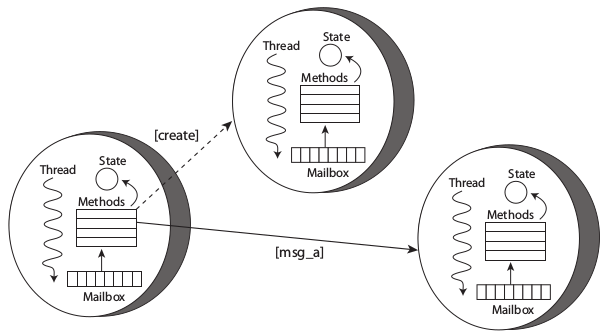
\includegraphics[width=140mm]{graphics/actor-messages.png}
\caption{Akcje w modelu aktorowym \autocite{karmani2009actor}}
\end{figure}

Aktory, w odróżnieniu od modelu współdzielonych zmiennych, nie dzielą między sobą wspólnych obszarów pamięci. Informacje w obliczeniach aktorów mogą być przekazywane, tylko i wyłącznie, poprzez wiadomości. Model ze współdzieloną pamięcią nie dostarcza żadnych mechanizmów abstrakcji i ukrywania informacji. Aby stwierdzić czy inny obiekt otrzymał dostęp lub zmodyfikował wykorzystywane zmienne wymagane jest zdefiniowanie odpowiedniego protokołu. Co więcej, nie można stwierdzić czy na danych nie zostały wykonane niewłaściwe lub wręcz niepożądane operacje. Jednym ze sposobów radzenia sobie z sytuacjami tego typu jest wykorzystywanie blokad i synchronizacji. Model aktorowy zakłada, że komunikacja pomiędzy aktorami nie jest synchroniczna, a akcje stanowią częściowy porządek. Nadchodzące wiadomości trafiają do skrzynki odbiorczej, gdzie czekają na przetworzenie. Wszystko to ma służyć zapobieganiu blokowania i przetrzymywania zasobów, co może doprowadzić do zakleszczeń (ang. \emph{deadlock}). Podstawową informacją zawartą w wiadomości jest istnienie innego \emph{aktora}. Jest to spowodowane tym, że \emph{aktor} A może skomunikować się z \emph{aktorem} B jedynie znając jego \emph{nazwę}. Tę wiedzę może posiąść jeśli otrzymał ją w chwili powstania lub poznał\\
w wyniku przetwarzania nadchodzących wiadomości. Co więcej, komunikacja jest transparentna. Pomimo ``świadomości'' istnienia innego aktora, nie jest znane jego położenie. Umożliwia to utworzenie systemu aktorów fizycznie rozproszonych pomiędzy wiele maszyn połączonych w sieć oraz dynamiczną rekonfigurację topologii \autocite{karmani2009actor, hewitt1977laws, agha86actors}.

\subsubsection{Akka Streams}\label{akka-streams}

\subsubsection{Reaktywne strumienie}\label{reaktywne-strumienie}

\subsubsection{React js}\label{react-js}

\subsubsection{Websocket}\label{websocket}

\subsection{Symulator wypłat z bankomatów}\label{symulator-wypux142at-z-bankomatuxf3w}

Cel: symulacja ma reprezentować realistyczne, naturalne rozkłady wypłat bankomatowych.

\subsubsection{Elementy symulacji}\label{elementy-symulacji}

\subsubsection{Karta}\label{karta}

\begin{itemize}
\tightlist
\item
  jest obiektem, który wypłaca pieniądze z bankomatu
\item
  posiada datę ważność
\item
  jest powiązana z bankiem / instytucją która ją wypuściła
\item
  może mieć różne waluty

  \begin{itemize}
  \tightlist
  \item
    czy karta na pewno może mieć różne waluty? jeśli ma inną walutę niż złotówki to jak przeliczamy? co z limitem wypłat
  \end{itemize}
\item
  może mieć limity
\end{itemize}

\paragraph{Bankomaty}\label{bankomaty}

\begin{itemize}
\tightlist
\item
  ma maksymalną pojemność
\item
  przynależy do banku / instytucji finansowej
\end{itemize}

\subsubsection{Parametry symulacji}\label{parametry-symulacji}

Symulacja musi być realistyczna, naturalna.

\begin{itemize}
\tightlist
\item
  ziarnistość symulacji: godzina
\item
  okres symulacji: rok
\item
  użytkownik ustala start i stop
\end{itemize}

Rozkłady muszą pokrywać cały okres symulacji.

\subsection{Wizualizacja wypłat na mapie}\label{wizualizacja-wypux142at-na-mapie}

Wizualizacja przedstawia pozycje bankomatów na mapie, ich stan sejfu oraz natężenie ruchu oraz błędy.
Udostępnia definiowanie konfiguracji symulacji.

Wyróżnianie bankomatów:

\begin{itemize}
\tightlist
\item
  wielkość kropki / kolor kropki - obciążenie bankomatu
\item
  stos pieniędzy, który maleje w miarę upływania pieniędzy w sejfie bankomatu
\end{itemize}

Po kliknięciu w bankomat na mapie pojawiają się szczegółowe informacje o stanie bankomatu:

\begin{itemize}
\tightlist
\item
  aktualne obciążenie bankomatu
\item
  zapasy pieniędzy
\item
  stan bankomatu - czy działa poprawnie, czy zaszła awaria
\item
  parametry symulacji danego bankomatu
\end{itemize}

Po prawej stronie znajdują się awarie, które zaszły w symulacji.
